\subsection{Hierarchical and Network Organization After Spectral Filtering}
\label{sec:network_organization}

The spectral analysis in Section~\ref{sec:rmt} showed that removing the dominant market mode reveals weaker but structured dependencies among groups of assets. We now examine whether these patterns also appear in the distance geometry of the correlation matrices. Hierarchical ordering provides a complementary representation of the same dependency structure, allowing localized organization to be compared across the original and RMT-filtered matrices.

\subsubsection{Hierarchical Organization of the Filtered Dependence Structure}
\label{sec:clustering}

Figure~\ref{fig:ordered_heatmaps} shows the correlation matrices after hierarchical ordering. The original matrix retains a broad positive background, consistent with the dominant collective component identified in the eigenspectrum. After spectral filtering, this common background is reduced and localized blocks become more visible. The group-mode representation is particularly informative because it emphasizes relative dependencies that remain after removal of the leading market component.

\begin{center}
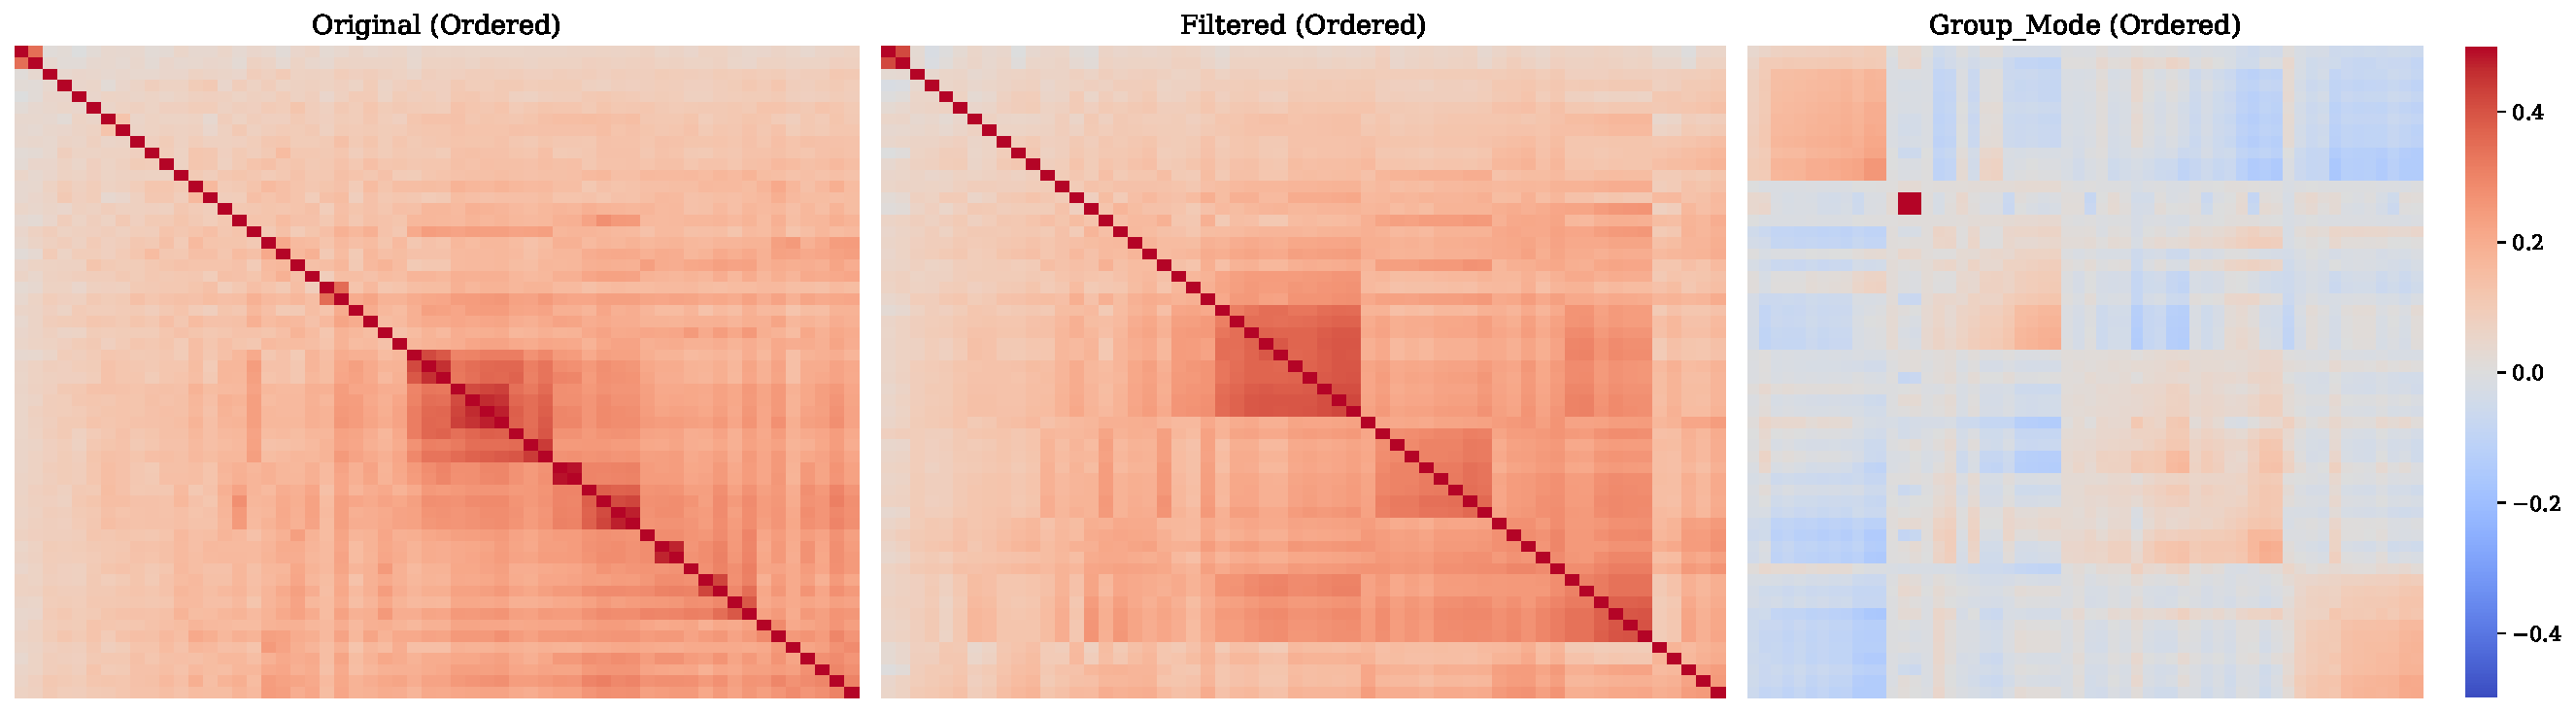
\includegraphics[
width=\linewidth,
height=0.72\textheight,
keepaspectratio
]{images/figure_10_ordered_heatmaps.pdf}
\captionof{figure}{Hierarchically ordered correlation matrices for the original and RMT-filtered structures. The common color scale highlights the reduction of broad market-wide co-movement and the emergence of more localized dependency patterns after spectral filtering.}
\label{fig:ordered_heatmaps}
\end{center}

The ordered matrices indicate that market-mode removal does not eliminate organization from the dependency structure. Instead, it changes its scale: the broad positive background becomes weaker while smaller blocks of relatively stronger and weaker relationships become easier to distinguish. These patterns are consistent with the heterogeneous compositions observed in the non-leading eigenvectors and suggest that part of the residual spectral structure is also expressed geometrically.

The corresponding hierarchical tree provides a more compact view of this organization. Figure~\ref{fig:dendrograms} shows the group-mode dendrogram obtained from Mantegna distances and average linkage. To shorten the long horizontal branches, the plotted merge heights use a monotone logarithmic transform; the tick labels report the original distances. Macro-sector colors are included only as an external reference for interpretation; the clustering procedure itself does not impose sector labels.

\begin{center}
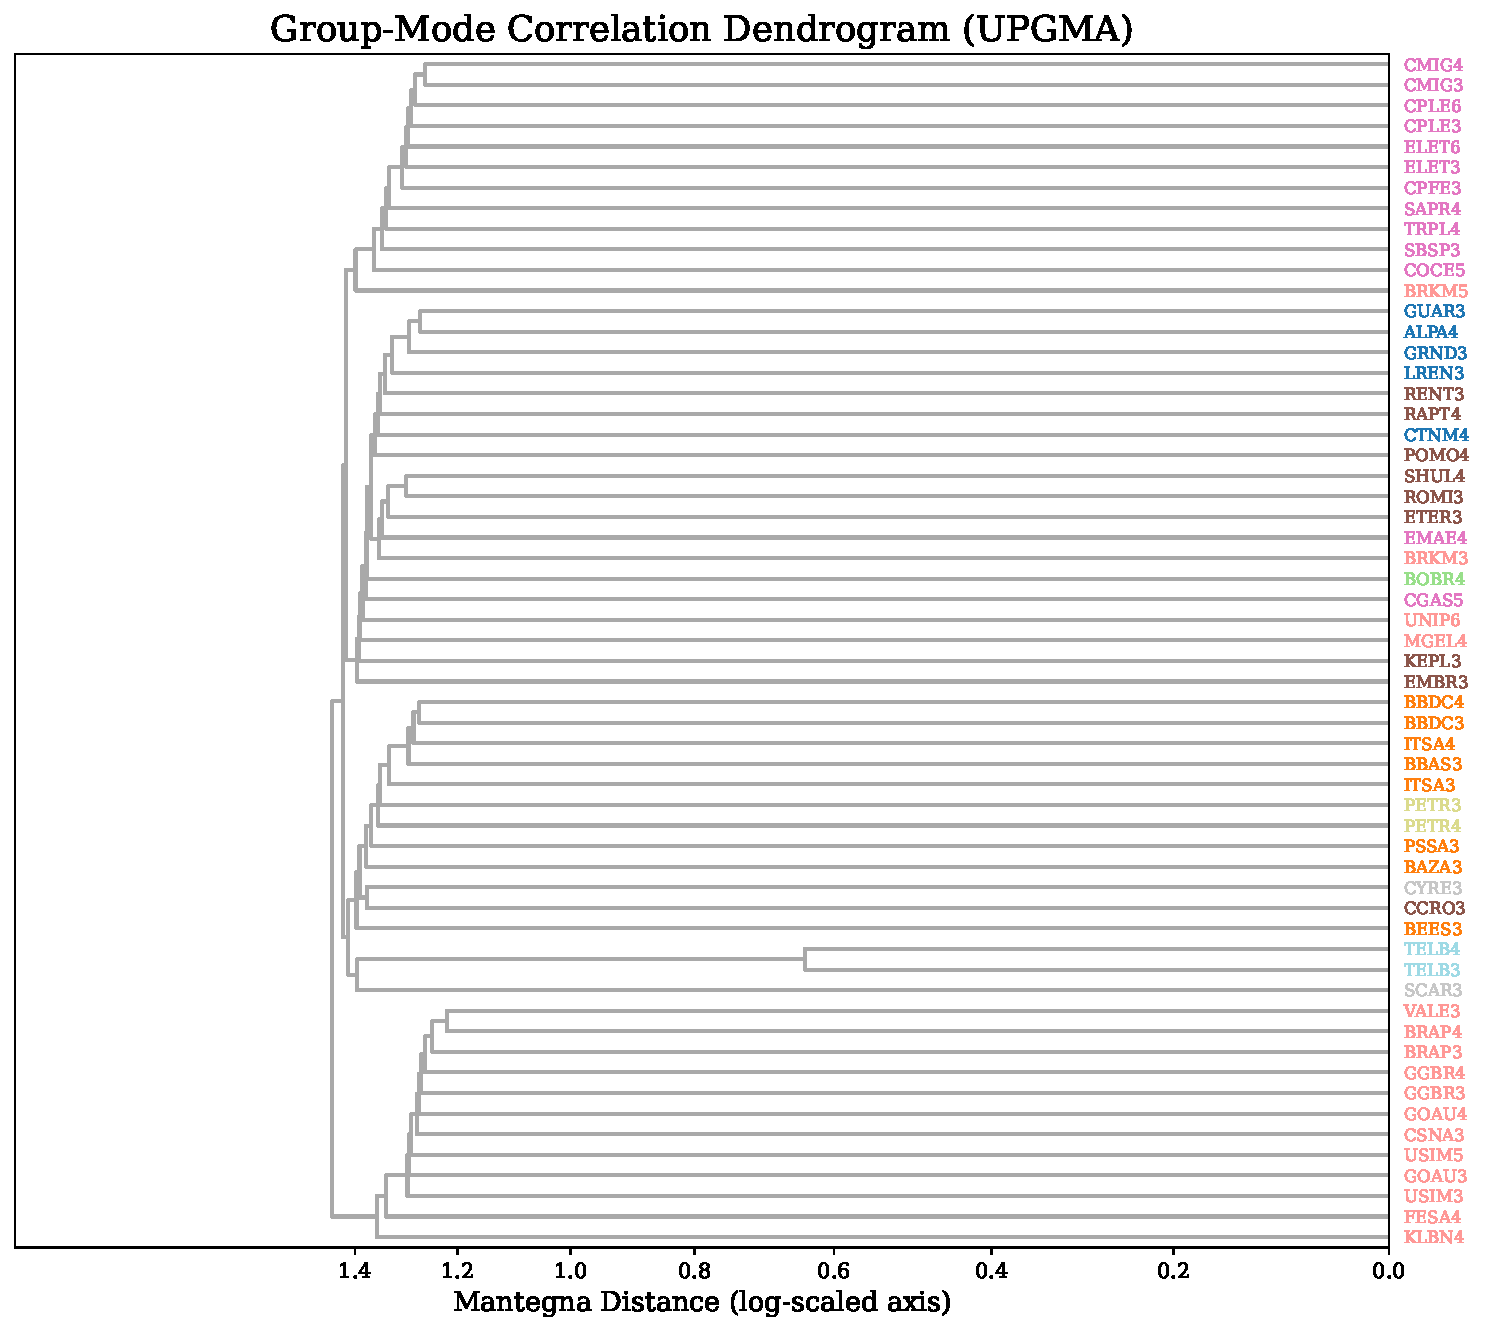
\includegraphics[
width=0.82\linewidth,
height=0.8\textheight,
keepaspectratio
]{images/figure_9_group_mode_dendrogram.pdf}
\captionof{figure}{Group-mode dendrogram obtained from Mantegna distances and average linkage. The horizontal axis uses a monotone log transformation, with tick labels in the original distance scale. The tree summarizes the dependency geometry remaining after removal of the dominant market mode; label colors indicate the initial macro-sector classification for comparison.}
\label{fig:dendrograms}
\end{center}

Table~\ref{tab:cophenetic_summary} compares how closely the hierarchical trees preserve the underlying distance structures.

\begin{center}
\captionof{table}{Cophenetic correlations for the original and RMT-filtered dependency structures.}
\label{tab:cophenetic_summary}
\begin{tabular}{lrr}
\toprule
Matrix & Assets & Cophenetic correlation \\
\midrule
Original & 58 & 0.950 \\
Filtered & 58 & 0.934 \\
Group-mode & 58 & 0.871 \\
\bottomrule
\end{tabular}
\end{center}


The supplementary Figure~\ref{fig:dendrograms_full_supplement} compares the original, filtered and group-mode trees side by side; it shows the additional geometric context for the focused group-mode tree in Figure~\ref{fig:dendrograms}. The original matrix has the highest cophenetic correlation, at 0.950, followed by the filtered matrix at 0.934 and the group-mode matrix at 0.871. The decline after market-mode removal indicates that the residual dependency structure is less accurately represented by a strictly hierarchical tree. This does not imply the disappearance of localized organization; rather, it suggests that the remaining geometry is more complex than the broad market-dominated structure observed in the original matrix.

The hierarchical analysis therefore provides two complementary findings. First, localized dependency patterns remain visible after removal of the dominant market component. Second, these relationships become less purely tree-like as the common market structure is removed. This motivates moving from hierarchical representations to graph-based filtering, where additional connections can be retained and the reorganization of hubs, local connectivity, and sectoral relationships can be examined directly.
